\documentclass[11pt, a4paper, doubleside]{Thesis}
\graphicspath{{./Pictures/}} % Specifies the directory where pictures are stored
\usepackage[utf8]{inputenc}
\setlength\parindent{24pt}

\usepackage{arydshln}%dibujar lineas verticales y horizontales
\usepackage{mathtools}
\usepackage{graphicx}
\usepackage[T1]{fontenc}
\usepackage{amssymb,graphicx}
\usepackage[utf8]{inputenc}
\usepackage{mathtools}
\usepackage{MnSymbol}
\usepackage{stmaryrd}
\usepackage{amsfonts}
\usepackage{amsmath}
\usepackage{amssymb}
\usepackage[all]{xy}
\usepackage{diagbox}
\usepackage[USenglish]{babel}

\newtheorem{theorem}{Theorem}[section]
\newtheorem{coro}{Corollary}[theorem]
\newtheorem{propo}{Proposition}[theorem]
\newtheorem{lemma}{Lemma}[theorem]
\newtheorem{defini}{Definition}[theorem]
\newtheorem{conje}[theorem]{Conjecture}
\newtheorem{prob}[theorem]{Problem}

\newtheorem{ejemp}[theorem]{Example}
\newtheorem{cond}[theorem]{Condition}
\newtheorem{nota}[theorem]{Note}
\newtheorem{notation}[theorem]{Notation}
\newtheorem{conv}[theorem]{Convention}

\newcommand{\E}{\mathbb{E}}
\newcommand{\F}{\mathcal{F}}
\newcommand{\R}{\mathbb{R}}
\newcommand{\Q}{\mathbb{Q}}
\newcommand{\N}{\mathbb{N}}
\newcommand{\Z}{\mathbb{Z}}
\renewcommand{\P}{\mathbb{P}}
\renewcommand{\G}{\mathcal{G}}
\renewcommand{\S}{\mathbb{S}}



\newenvironment{cajita}
    {\begin{center}
    \begin{tabular}{|p{0.9\textwidth}|}
    \hline\\
    }
    { 
    \\\\\hline
    \end{tabular} 
    \end{center}
    }  
    

\usepackage[table]{xcolor}
\definecolor{Blue}{HTML}{006699}
\definecolor{Green}{HTML}{4F9C45}

\providecommand{\abs}[1]{\lvert#1\rvert}

\title{\ttitle} % Defines the thesis title - don't touch this

\begin{document}

\frontmatter % Use roman page numbering style (i, ii, iii, iv...) for the pre-content pages

\setstretch{1.3} % Line spacing of 1.3

% Define the page headers using the FancyHdr package and set up for one-sided printing
\fancyhead{} % Clears all page headers and footers
\rhead{\thepage} % Sets the right side header to show the page number
\lhead{} % Clears the left side page header

\pagestyle{fancy} % Finally, use the "fancy" page style to implement the FancyHdr headers

\newcommand{\HRule}{\rule{\linewidth}{0.5mm}} % New command to make the lines in the title page

% PDF meta-data
\hypersetup{pdftitle={\ttitle}}
\hypersetup{pdfsubject=\subjectname}
\hypersetup{pdfauthor=\authornames}
\hypersetup{pdfkeywords=\keywordnames}

%----------------------------------------------------------------------------------------
%	TITLE PAGE
%----------------------------------------------------------------------------------------

%\begin{titlepage}
%\phantom{Hola}
%\end{titlepage}
%\clearpage

%----------------------------------------------------------------------------------------
%	Frase conmovedora
%----------------------------------------------------------------------------------------

\pagestyle{empty} % No headers or footers for the following pages

\null\vfill % Add some space to move the quote down the page a bit
\begin{flushright}
\textit{Fahre fort, übe nicht allein die Kunst, sondern dringe auch in ihr Inneres; sie verdient es, denn nur die Kunst und die Wissenschaft erhöhen den Menschen bis zur Gottheit.
}
\end{flushright}
\begin{flushright}
\textit{Do not merely practice your art, but penetrate into its interior; it deserves that, because only art and science exalt man to divinity.
}
\end{flushright}


\begin{flushright}
Ludwig van Beethoven
\end{flushright}

\vfill\vfill\vfill\vfill\vfill\vfill\null % Add some space at the bottom to position the quote just right
\clearpage


%----------------------------------------------------------------------------------------
%	ACKNOWLEDGEMENTS
%----------------------------------------------------------------------------------------

%\setstretch{1.3} % Reset the line-spacing to 1.3 for body text (if it has changed)

%\acknowledgements{\addtocontents{toc}{\vspace{1em}} % Add a gap in the Contents, for aesthetics
%}
%\clearpage % Start a new page

%----------------------------------------------------------------------------------------
%	LIST OF CONTENTS/FIGURES/TABLES PAGES
%----------------------------------------------------------------------------------------

\pagestyle{fancy} % The page style headers have been "empty" all this time, now use the "fancy" headers as defined before to bring them back

\lhead{\emph{Indice}} % Set the left side page header to "Contents"
\tableofcontents % Write out the Table of Contents

%\lhead{\emph{List of Figures}} % Set the left side page header to "List of Figures"
%\listoffigures % Write out the List of Figures

%\lhead{\emph{List of Tables}} % Set the left side page header to "List of Tables"
%\listoftables % Write out the List of Tables

%----------------------------------------------------------------------------------------
%	RESUMEN PAGE
%----------------------------------------------------------------------------------------

%\begin{Resumen}


%\vspace{5cm}

%\textit{Palabras clave:} 
%\end{Resumen}

%----------------------------------------------------------------------------------------
%	ABSTRACT PAGE
%----------------------------------------------------------------------------------------

\begin{abstract}

%In this work we propose the use of the Radó graph and the Erdös Rényi model for random graphs to study a rigidity phenomenon in graphs called rigid expansions. We review the motivation to stud
rg
%The goal is to do it in the curve graph associated to a surface $S$, we will show the conditions under which is possible to do it in a simple probabilistic model.

\end{abstract}

%----------------------------------------------------------------------------------------
%	ABBREVIATIONS
%----------------------------------------------------------------------------------------

%\clearpage % Start a new page

%\setstretch{1.5} % Set the line spacing to 1.5, this makes the following tables easier to read

%\lhead{\emph{Abbreviations}} % Set the left side page header to "Abbreviations"

%\listofsymbols{ll} % Include a list of Abbreviations (a table of two columns)
%{
%\textbf{LAH} & \textbf{L}ist \textbf{A}bbreviations \textbf{H}ere \\
%\textbf{Acronym} & \textbf{W}hat (it) \textbf{S}tands \textbf{F}or \\
%}

%----------------------------------------------------------------------------------------
%	SYMBOLS
%----------------------------------------------------------------------------------------

\clearpage % Start a new page

\lhead{\emph{Symbols}} % Set the left side page header to "Symbols"

%\listofnomenclature{ll}{ % Include a list of Symbols (a three column table)
%$K\RFD L$ & Retracto por deformación fuerte. \\
%}

%----------------------------------------------------------------------------------------
%	DEDICATION
%----------------------------------------------------------------------------------------

\setstretch{1.3} % Return the line spacing back to 1.3

\pagestyle{empty} % Page style needs to be empty for this page

\dedicatory{} % Dedication text

\addtocontents{toc}{\vspace{2em}} % Add a gap in the Contents, for aesthetics



%----------------------------------------------------------------------------------------
%	THESIS CONTENT - CHAPTERS
%----------------------------------------------------------------------------------------

\mainmatter % Begin numeric (1,2,3...) page numbering

\pagestyle{fancy} % Return the page headers back to the "fancy" style

% Include the chapters of the thesis as separate files from the Chapters folder
% Uncomment the lines as you write the chapters
% Introducción
\chapter*{Introduction} % Main chapter title

\label{Intro} % For referencing the chapter elsewhere, use \ref{Chapter1} 

\lhead{\emph{Introduction}} % This is for the header on each page - perhaps a shortened title

%----------------------------------------------------------------------------------------
%----------------------------------------------------------------------------------------
%	INTRODUCTION
%----------------------------------------------------------------------------------------

The curve graph $\Gamma(S)$ associated to a surface $S$ appears naturally in the study of $Mod(S)$, the mapping class group of $S$, which is a central subject in contemporary mathematical research. We are interested in a rigidity concept of this graph; in general, the idea behind rigidity phenomena is to describe morphisms among objects using their structure.

The folkloric version of rigidity in the $Mod(S)$ context is that if we consider $X$ and $Y$, under suitable conditions, then every homomorphism $Mod(X) \to Mod(Y)$ will be induced by a manipulation of the underlying surfaces.

Ivanov sketched in \cite[Ivanov 97]{celebratedIvanov} the proof that every automorphism of $C(S)$ (the flag complex of $\Gamma(S)$), is induced by a self-homeomorphism of $S$. This argument is the favorite in the literature due to its simplicity and resemblance to proofs of other rigidity results.

A research line lead by Aramayona and Leininger propose the idea of \textit{rigid sets}, which can be interpreted as a subset \textit{that allows to extend a local notion of rigidity to global one}. In the aim of finding large rigid sets, in \cite[Aramayona, Leininger 16]{finiteRigidSetsJA} there's the proof of the existence of an increasing sequence of finite rigid sets that exhaust the curve graph. For this, they proposed a method called \textbf{rigid expansions}.

Rigidity in graphs is, regardless of its interpretation in the curve graph, an interesting phenomenon by it self. Due to the discrete nature of rigid expansions is reasonable to seek for a probabilistic approach; our goal is to address this particular path.

We want to answer the rather vague question: \textit{How \textbf{common} is rigidity in graphs}, specifically by answering \textit{how rigid expansions \textbf{usually} behave}. Also, the aim of the thesis is to review the feasibility of \textit{studying the curve complex of a surface from a probabilistic point of view.}

Probabilistic models give formal meaning to words like "common" or "usually" and in rigidity's panorama allow us to study such complex phenomenon. We will analyze the conditions under which these models can fit the known properties of the curve graph.

In chapter one, we motivate the study of the curve graph and review the most important properties of it. Then, we will introduce rigidity within the context of Graph theory.

In the second chapter, we propose the study of rigidity from the stochastic point of view through the Radó graph and the Erdös-Rényi model. In the aim to study the curve graph of a surface with a simple model, we justify that the genus of the surface cannot be finite. Thus, we end up with an asymptotic probabilistic analogue to the result due to Bering and Gaster, which asserts that the Radó graph embeds into the curve graph $C(S)$ of a surface $S$ if and only if $S$ has infinite genus.

Finally, we made a computational implementation of the algorithm to do rigid expansions. With the corresponding optimizations that the method require, we were able to take a closer look to rigidity phenomena.
% Chapter 1

\chapter{The curve complex of a surface} % Main chapter title

\label{Chapter1} % For referencing the chapter elsewhere, use \ref{Chapter1} 

\lhead{Chapter 1. \emph{The curve complex of a surface}} % This is for the header on each page - perhaps a shortened title

%----------------------------------------------------------------------------------------

The study of surfaces in a strictly topological viewpoint has made us to forgot significant information about them. A way to revert this is to attach a group to it, the \textbf{mapping class group} of the surface, it's denoted by $Mod(S)$ and encode the \textit{symmetries} of the surface. This group is defined as the set of isotopy classes of orientation-preserving homeomorphisms of $S$. In the first section of this chapter we'll give the formal definition of this group and establish the very important role of this concept in Mathematics. 

There's a widely accepted idea that Mathematics can be thought as a story of groups and that groups as men are judged by their actions. Taken this point of view, the \textbf{curve complex} of the surface, denoted by $C(S)$ appears naturally in the study of $Mod(S)$ as an object in which this group acts. It is a simplicial complex that encodes intersection patterns of simple closed curves in $S$. We will focus part of the discussion in the relationship between the algebraic structure of $Mod(S)$ and the combinatorial topology of $S$.

Many of the progress in understanding $Mod(S)$ has been possible by a well-known comparison among two very important classes of groups: arithmetic groups and mapping class groups. In this parallelism panorama arises the desire for an equivalent, until some extent, of the Margulis Superrigidity for mapping class groups.

Rigidity phenomena called mathematicians attention because it uses the structure of the objects to describe morphisms between them. In the aim to extend the results of rigidity in simplicial maps there's an approach called \textit{rigid expansions} see \cite[Aramayona 16]{rigidExpJA} and \cite[Hernandez 16]{rigidExpJH}, which allows us to generate rigid sets from an initial one. We'll take particular interest in this point of view because of its combinatorial nature and therefore its compatibility with the stochastic background that will be settled in the following chapter.

Many results and definitions in this chapter where extracted from \cite[Farb]{Farb}. They're quite popular and equivalents can easily be find in the literature, however they are written here to establish nomenclature. Familiarity with basic concepts will be assumed.

\section{Mapping class group of a surface}

We have the following fundamental, well-known result about surfaces.

\begin{theorem}[Classification of surfaces]\label{CST}
Any closed, connected, orientable surface is homeomorphic to the connect sum of a 2-dimensional sphere with $g \geq 0$ tori. Any compact, connected, orientable surface is obtained from a closed surface by removing $b \geq 0 $ open disks with disjoint closures. Even more, the set of homeomorphism types of compact surfaces is in bijective correspondence with the set $\{ (g, b) : g, b \geq 0\}$.
\end{theorem}

We are so familiarized whit this result that we forget what it's saying. It seems like, in the eyes of a topologyst, there's nothing much interesting about surfaces, but this is because we are forgetting all the geometric information about them. $Mod(S)$ helps to recover this data, the magic happens when this group acts on the \textbf{Teichmüller space} of $S$, that is the space of hyperbolic metrics on $S$ up to isotopy. A central result is that this action results to be properly discontinuous and the quotient space $M(S) = Teich(S)/ Mod(S)$ is the \textbf{moduli space of Riemannian surfaces} homeomorphic to $S$. The space $M(S)$ is a essential object in mathematics and the group $Mod(S)$ encodes most of the topological features of $M(S)$.

$Mod(S)$, $Teich(S)$, and $M(S)$ can be found in a lot of different contexts in mathematics: hyperbolic geometry, algebraic geometry, combinatorial group theory, symplectic geometry, 3-manifold theory, dynamics and so on. The algebraic structure of $Mod(S)$, the geometry of $Teich(S)$, and the topology of $M(S)$ are just the strands which are used to weave the rich tapestry of the combinatorial topology of the surface.

Before we continue, let's establish some nomenclature. The $g$ in \ref{CST} is called the \textit{genus} of the surface and the $b$ is the number of \textit{boundary components}. One way to obtain a non-compact surface from a compact one is to remove $m$ points from the interior of it; in this case, we say that the resulting surface has $m$ punctures. For now on, unless otherwise specified, we will be thinking in compact, connected, oriented surfaces that are possibly punctured (in this case they ceases to be compact). We can therefore specify our surfaces by the triple $(g, b, m)$. We will denote by $S_{g,m}$ a surface of genus $g$ with $m$ punctures and empty boundary; such a surface is homeomorphic to the interior of a compact surface with $m$ boundary components. Also, for a closed surface of genus $g$, we will abbreviate $S_{g,0}$ as $S_{g}$ and $\partial S$ will denote the (possibly disconnected) boundary of $S$.

There are a number of definitions for the mapping class group of a surface. We will be working with the following:

\begin{defini}
Let $S$ be a surface, the \textbf{mapping class group} of $S$, denoted by $Mod(S)$ is the following quotient:
$$Mod(S)=Homeo^{+}(S)/Homeo_{0}(S)$$
where $Homeo^{+}(S)$ is the group of orientation-preserving, homeomorphisms of $S$, that are the identity on the boundary, this group can be endowed with the compact-open topology. $Homeo_{0}(S)$ is the subgroup formed by homeomorphisms of $S$ which are isotopic to the identity, i.e. the connected component of the identity with this topology.
\end{defini}

We could consider diffeomorphisms instead of homeomorphisms, or homotopy classes instead of isotopy classes, this will result in isomorphic groups, see \cite[Farb 41]{Farb} for details in why we can do this. Summarizing, we can find the following variations in the definition of $Mod(S)$:

\centerline{\begin{tabular}{ rcl }
$Mod(S)$ & $=$ & $\pi_{0}(Homeo^{+}(S, \partial S))$\\
 & $\approx$ & $Homeo^{+}(S,\partial S)/\textit{homotopy}$\\
 & $\approx$ & $\pi_{0} (\textit{Diff}^{+}(S,\partial S))$\\
\end{tabular}}

where $\textit{Diff}^{+}(S, \partial S)$ is the group of orientation-preserving diffeomorphisms of $S$ that are the identity on the boundary and can be taken to be either smooth homotopy relative to the boundary or smooth isotopy relative to the boundary.

A lot of work had been made to describe the types of elements in $Mod(S)$. Thanks to the Thurston's classification theorem there's a characterization of the homeomorphisms of a compact orientable surface. This classification is useful to describe the curve complex which will be analyzed in the next section.

\subsection{Nielsen–Thurston classification}
Given a homeomorphism $f: S \to  S$, there is a map $g$ isotopic to $f$ such that at least one of the following holds:

\begin{itemize}
\item $g$ is periodic, i.e. some power of $g$ is the identity;
\item $g$ preserves some finite union of disjoint simple closed curves on $S$ (in this case, g is called reducible); or
\item $g$ is pseudo-Anosov.
\end{itemize}

The definition of a \textbf{pseudo-Anosov map} relies on the notion of a measured foliation which is a geometric structure on $S$. It consists of a singular foliation and a measure in the transverse direction (i.e. that it's constant in transverse arches). For the full definition of pseudo-Anosov elements and the proof of this theorem we can refer to \cite[Farb, Chapter 13]{Farb}

The study of mapping class groups it's a wide and challenging area of the mathematics by it self. It's outside of the interests of this thesis to review the details and repercussions of this vastly field. Yet, there are a number of known properties of $Mod(S)$ that it would be nice to have in mind in further work, although different tools that the ones here presented might be required.

\begin{itemize}
\item Finitely generated and presented
\item It has a subgroup of finite index which doesn't have torsion.
\item $Mod(S_{g,m}) \cong Out(\pi_{1}(S_{g,m})$
\item $H_{1}(Mod(S_{g,m}), \Z) = 1$ when $(g\geq3, m=0)$
\end{itemize}

\section{Curve complex}

\subsection{Simple closed curves}

\begin{defini}
A \textbf{closed curve} in a surface $S$ is a continuous map $\S^{1}\to S$, it's called \textbf{simple} if the map is injective. We'll usually identify a closed curve with its image in $S$. A closed curve is called \textbf{essential} if it's not homotopic to a point, a puncture, or a boundary component.
\end{defini}
Among the adjectives that a curve can acquired we have the following:
\begin{itemize}
    \item $\alpha$ is \textbf{separating}, if $S-\alpha$ has two components, otherwise it is called \textbf{non separating}.
    \item it's called \textbf{essential} if no component of $S- \alpha$ is a disk.
    \item it's \textbf{non-peripheral} if no component of $S - \alpha$ is an annulus. 
\end{itemize}

We are interested in \textbf{essential} and \textbf{non-peripherial} curves, they will be assumed in this sense, unless otherwise specified.

The idea behind the construction of the curve complex is to stratify the set of homotopy classes of curves on a surface. For this to make sense we define the \textbf{geometric intersection number} between free homotopy classes $a$ and $b$ of simple closed curves in a surface $S$. This is defined to be the minimal number of intersection points between a representative curve in the class $a$ and a representative curve in the class $b$:
$$i(a,b) = min \{ |\alpha \cap \beta| : \alpha \in a, \beta \in b \}$$
Sometimes it'll be convenient to adopt a slight abuse of notation by writing $i(\alpha, \beta)$ for the intersection number between the homotopy classes of simple closed curves $\alpha$ and $\beta$. It's useful to think that this number can be calculate by finding representatives $\alpha$ and $\beta$ that realize the minimal intersection in their homotopy classes, so that $i(a, b) = |\alpha \cap \beta|$. When this is the case, we say that $\alpha$ and $\beta$ are in minimal position. Although the geometric intersection number is a useful and intuitive invariant it's not always easy to compute, whenever this is the case we can appeal to the algebraic intersection number. For a further discussion of this see \cite[Farb]{Farb}

\subsection{The curve complex}

\begin{defini}
The \textbf{curve graph} $\Gamma(S)$ of a surface $S$, is constructed by the following data:
\begin{itemize}
\item \textbf{Vertices}. There's a vertex in $\Gamma(S)$ for every isotopy class of essential closed curves in $S$.
\item \textbf{Edges}. There's an edge between the corresponding vertices of isotopy classes $a$ and $b$ whenever $i(a,b)=0$.
\end{itemize}
\end{defini}

\begin{defini}
The \textbf{curve complex of the surface}, $C(S)$ is defined to be the flag complex of the graph of curves just defined.
\end{defini}

\section{Properties of the curve complex}
The goal of this sections is to enumerate known properties of the curve complex that will be useful to establish the appropriate parameters in the probabilistic model. Notice that the construction of the curve complex is completely given by the curve graph, the probabilistic model will work in the same sense and that's why we'll be jumping between the complex to the graph whenever it's more convenient. Let's keep in mind the following exceptional cases; they are the responsible for the conditions stated in the hypothesis of the following theorems for $g$ and $n$. For $ S^2, S_{0,1}, S _{0,2}, S_{0,3} $ the curve complex is empty and for  $ T^{2} $, $ S_{1,1}$ and $ S_{0,4}$ is a countable disjoint union of points.

\subsection{Cardinality of the number of vertices}
\begin{theorem}
If $g\geq 1$ or $n\geq 4$ then the set of vertices in $C(S_{g,n})$ is countably infinite.
\end{theorem}

It's well known that for $T^{2}$ there's an explicit identification for the isotopy classes of essential curves with the rational numbers. In this case there aren't disjoint curves, this easy to believe by looking the following picture.
\vspace{1cm}
\begin{figure}[h!]
	\centering
	\includegraphics[scale=0.7]{Figures/Torus.png}
	\caption{$T^{2}$ with representatives of typical elements of curves}
\end{figure}

This identification can be seen as the induction basis and then the induction step over $g$ comes from splitting the surface, by the induction hypotheses none of the resulting surfaces can have a non-countable number of curves.

\subsection{Connectivity}
\begin{theorem}
If $3g+n\geq 5$, then $C(S_{g,n})$ is connected.
\end{theorem}

The $3g+n\geq 5$ hypothesis means that the result exclude the problematic cases which we already discuss. To proof this theorem we can show that for any two isotopy classes $a$ and $b$ of simple closed curves in $s_{g,n}$ exists a sequence of isotopy classes
$$a=c_{1},\dots,c_{k}=b$$
where $i(c_{i},c_{i+1})=0$, this can be done proceeding by induction over $i(a,b)$ The proof of this theorem can be found in \cite[Farb p.~93]{Farb} 

\subsection{Locally infinity}
\begin{theorem}
If $3g+m\geq 5$, then $C(S_{g,n})$ is locally infinity.
\end{theorem}
The idea behind the proof of this theorem is that given any $\alpha \in C(S)$ we can construct a family of isotopy classes of curves which are disjoint to $\alpha$. The following picture gives us an intuitive idea on how to do this.
\vspace{1cm}
\begin{figure}[h!]
	\centering
	\includegraphics[scale=0.5]{Figures/Locally-infinite.png}
	\caption{$S_{3}$ with typical representative curves which provide the locally infinity property}
\end{figure}

For the complete argument let $\alpha$ be any simple closed curve on $S$, the surface $S-\alpha$ which we obtain by cutting $S$ open along $\alpha$ contains at least one connected component of Euler characteristic at most $-2$, and such a component contains infinitely many distinct homotopy classes of simple closed curves which viewed as curves in $S$ are disjoint from $\alpha$ 

\subsection{Clique number}
A \textbf{clique} in a graph $G$ is a complete subgraph of $G$. The clique number $cl(G)$ of a graph $G$ is the maximum order of a clique of $G$.

\begin{theorem}
If $3g+n\geq 5$, then $3g - 3 + m$ is the clique number of $C(S_{g,m})$.
\end{theorem}

 This is because $3g-3+m$ is the number of curves in a pants decomposition of $S$, i.e. a maximal collection of disjoint mutually not freely homotopic essential simple closed curves which decompose $S$ into $2g-2+m$ open subsurfaces homeomorphic to a thrice punctures sphere, making the dimension of $C(S)$ equals $3g-4+m$, for a full proof of this well-known fact refer to \cite[Hatcher]{Pants}
 
\vspace{1cm}
\begin{figure}[h!]
	\centering
	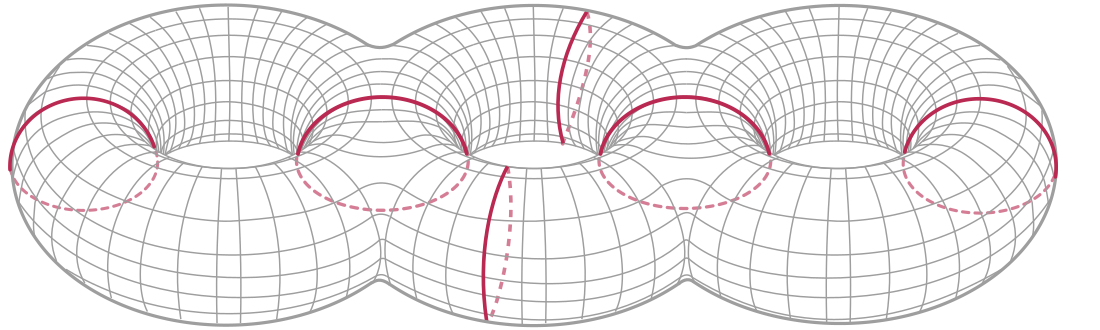
\includegraphics[scale=0.4]{Figures/Pantalones.png}
	\caption{Exemplification of a panths decomposition of a surface}
\end{figure}

\subsection{Infinite Diameter}
\begin{theorem}
If $3g+m\geq 5$ then $diam(C(S)) = \infty$
\end{theorem}

The proof for this theorem relies on the fact that for any psuedo-Anosov element $h \in Mod(S)$, any $\gamma \in V(C(S))$ and any $k\in \Z$

$$d_{C}(h^{k}(\gamma), \gamma) \geq c|k|$$
 
For details on the proof refer to \cite[Masur and Minsky]{Masur}

The curve complex is a fundamental tool in the study of the geometry and combinatorial topology of the surfaces. It's interesting and challenging enough to study $C(S)$ by its own. There are a number of known properties of it that it would be nice to have in mind to refine the probabilistic model in further work.

\begin{enumerate}
\item C(S) is hyperbolic
\item In the infinite case $diam(C(S))= 2$
\item There's an isomorphism between $Mod(S)$ and $Aut(C(S))$ (except when $(g,m) \in \{(1,2), (1,1), (2,0), (0,4)\}$
\end{enumerate}

\section{Rigidity}

As we talk in the introduction of the chapter, rigidity appears in the mapping class group context in light of its comparison with arithmetic groups. In \cite[Aramayona, S.]{rigidityJA} we can find a survey on the search of an analogue for the Margulis Superrigidity theorem. They propose three different perspectives: a Lie theoretical, a geometric and a folkloric one.

The Lie theoretic version of superrigidity says that every homomorphism $Mod(X) \to Mod(Y)$ is induced by a homomorphism $\textit{Diff}_{c}(X) \to \textit{Diff}_{c}(Y)$ between the associated groups of diffeomorphisms with compact support disjoint from the boundary.

A direct formulation of geometric superrigidity cannot hold when the moduli space it's endowed with any reasonable metric. However, there are ways to turn this around, saying that every (irreducible) homomorphism between mapping class groups induces a holomorphic map between the corresponding moduli spaces.

The folkloric version of Mostow and Margulis superrigidity claims that the only homomorphisms between lattices are the “obvious ones”, in the $Mods(S)$ context this will mean that if we consider $X$ and $Y$, under suitable conditions, then every homomorphism $Mod(X) \to Mod(Y)$ will be induced by a manipulation of the underlying surfaces. 

A result due to Ivanov asserts that every automorphism of $C(S)$ is induced by a self-homeomorphism of $S$. This argument is the favorite in the literature to do the bridging among this two worlds; it is easy, beautiful and parallels the proof of the Mostow Rigidity theorem in higher rank, replacing the Tits building by the curve complex. A lot of work has been developed trying to generalize this result, in \cite[J. Hernández]{rigidExpJH} we can find a summary of the state of the art of this pipeline with the appropriate bibliographic references. 

There's a method to expand subgraphs developed in \cite[Aramayona, Leininger]{rigidExpJH} which can be used to obtain new results concerning edge-preserving maps. We'll take particular interest to this method due to it's combinatorial nature.

\begin{defini}
Let $\Gamma$ be a simplicial graph and let $H<\Gamma$ be a vertex-induced subgraph. A function $f:y\to \Gamma$ is \textbf{locally injective} if $f|_{star(v)}$ is injective for all $v \in V(y)$. 
\end{defini}

\begin{nota}
Remember, $star(v)$ is the vertex-induced subgraph with vertices $\{ v \} \cup N(v)$ ($v$ plus its neighborhood).
\end{nota}

\begin{defini}
$H<\Gamma$ is \textbf{rigid} if every locally injective function defined in $H$ can be extended to an automorphism of $\Gamma$. \end{defini}

A vertex $v \in V$ in a graph it's called to be uniquely determined by $A\subset V(G)$, denoted $v=<A>$, if $v$ is the unique neighbor of every element of $B$, i.e.

$$ \{ v \} = \bigcap_{w\in B} lnk(w) $$

\begin{defini}
The first rigid expansion of $Y\subset \Gamma$ is the vertex-induced subgraph whose vertices are
$$ V(Y) \cup \{ v\in V(\Gamma) :  \exists A \subset V(Y) \text{ where } v = <A>  \}$$
\end{defini}

To motivate the computational approach, it would be nice to have conditions which determine whether a subcomplex is rigid or not. So far we know that there aren't non-trivial necessary conditions to check rigidity, i.e. other than connectivity there's not much else.
% Chapter 2

\chapter{Rigidity in random graphs} % Main chapter title

\label{Chapter2} % For referencing the chapter elsewhere, use \ref{Chapter1} 

\lhead{Chapter 2. \emph{Rigidity in random graphs}} % This is for the header on each page - perhaps a shortened title

%----------------------------------------------------------------------------------------

The use of the probabilistic method in discrete mathematics has become a prominent idea in the area in recent times. It provides existence proofs where objects have certain desirable properties and the construction of explicit examples is challenging. This has been just the beginning of the use of probabilistic tools within a deterministic context.

Complex topological spaces arise quite naturally in a lot of scientific contexts. Probability theory implements different approaches to model those spaces; even in complex configurations, it can be possible by doing approximations, to study topological invariants. In this sense, stochastic topology can be thought of as a tool for topology in the same sense as statistical mechanics is used to studying a macroscopic physical system when classical mechanics finds these systems too complicated to solve. 

Stochastic topology finds its early motivation in applied problems. Nevertheless, in recent articles, it has been used to provide deeper insight into theoretical questions. For example, with probabilistic analogs of very classical topology conjectures, like Whitehead's Asphericity Conjecture \cite[Costa, Faber 15]{Costa15}.

Probability theory can help us understand the ubiquity of certain mathematical phenomena. For example, \textit{many} simplicial complexes and posets which arise from combinatorial constructions are homotopy equivalent to a wedge of spheres, or that hyperbolicity is \textit{common} in random groups. With Probability theory, we can give formal meaning to these expressions.

In this chapter, we review rigid expansions in simple probabilistic models. Afterward, we analyze the feasibility of modeling the curve graph using these proposals.

Familiarity with basic concepts in probability theory such as probability spaces, random variables, and basic theorems are assumed.

\section{Models for random graphs}

\subsection{The Radó graph}
Let $0 < p < 1$ be fixed, $\G(\N, p)$ is the probability space which consists of all graphs with vertex set $\N$, whose edges are chosen independently with probability $p$. In other words, a random graph $G \in \G(\N,p)$ is a collection $(X_{ij}) = \{ X_{ij} : 1 \leq i < j\}$ of independent $Bernoulli(p)$ r.v., where a pair $ij$ is an edge of $G$ if and only if $X_{ij} = 1$.

Erdős and Rényi proved in \cite[Erdős, Rényi 63]{RadoUnique}, that every countably infinite random graph is isomorphic to the \textbf{Radó graph}. A construction of this graph can be done using binary numbers; identify the vertices of the graph with the natural numbers and then every edge appears between vertices $x$ and $y$ in the graph (assuming $x < y$) whenever the $x$-th bit of the binary representation of $y$ is nonzero. This means, for example, that all odd-numbered vertices will be neighbors of vertex $0$, and that the larger neighbors of vertex $1$ are all vertices with numbers congruent to $2$ or $3$ mod $4$.

\begin{figure}[h!]
	\centering
	\includegraphics[scale=0.7]{Figures/Rado-graph.png}
	\caption{Binary construction of the Radó graph.}
\end{figure}

\subsection{Erdős-Rényi model}
The Erdős-Rényi model for random graphs is the finite version of the Radó graph. In this model, the parameter $p$ is usually taken as a function of $n$. This provides, unlike the past model, a variety of graphs when $n$ tends to infinity.

\begin{defini}
Denote by $\G(n,p)$ to the probability space formed by all the graphs of $n$ vertices and probability measure 
$$ \P\Big(G\in \G(n,p)\Big) = p^{k} (1-p)^{\binom{n}{2}-k},$$
where $k$ is the number of edges in $G$, the $\sigma$-algebra is given by the power set.
\end{defini}

Note: There is a variation of the model, where we rather choose randomly exactly $m$ edges among the $\binom{n}{2}$ possible.

We can also think this model like $\binom{n}{2}$ i.i.d. $Bernoulli(p)$ that represent the edges. From this, we can immediately get some properties of the degree of a vertex $v$.

\begin{itemize}
\item The probability that a given vertex $v$ has degree $k$ is given by
$$b(k; n-1,p) = \binom{n-1}{k} \cdot p^{k} \cdot (p-1)^{n-k-1}.$$
\item The expected degree is $(n-1)\cdot p$.
\item The variance of this degree is $(n-1)\cdot (1-p) \cdot p$.
\end{itemize}

The degree distribution can be helpful to do optimizations in the rigid expansions algorithms. This is outlined in the next chapter.

\section{Rigid expansions}

 We will focus on the rigidity calculations for the finite case. Then, we will analyze what happens when $n$ tends to infinite. For this, we need to compute the probability that the following events occur.

\begin{enumerate}
\item Let us call $E_{m}$ to the event when $v=\langle A_{m}\rangle$, where $v$ is a vertex and $A_{m}$ a subset of vertices of size $m$.
\item $A_k$ generates a rigid expansion.
\item $A_k$ generates a rigid expansion with $s$ new elements.
\end{enumerate}

For the calculations concerning the first event, take a look at the following figure.

\begin{figure}[h!]
	\centering
	\includegraphics[scale=1]{Figures/uni.png}
	\caption{Probability of uniquely determined vertices.}
\end{figure}

If $\langle A_{m} \rangle = v$, there is a edge between $v$ and every vertex in $A$, and none of the remaining $n-m-1$ vertices is also connected to every vertex in $A$, i.e.
$$\P (E_m) := \P(\langle A_{m}\rangle = v) = p^{m}(1-p^{m})^{n-m-1}.$$
Using the \texttt{networkx} library in \texttt{python} we reproduce the following experiment:

\begin{cajita}
\textbf{Uniquely determined vertex experiment.} Let $n,p,m$ be fixed.
\begin{enumerate}
\item Generate an Erdős-Rényi graph $G\in \G(n,p)$ with labeled vertices.
\item Excluding the $n$-th vertex, take a random subset of vertices of size $m$.
\item Verify if this subset uniquely determine the $n$-th vertex.
\end{enumerate}
\end{cajita}

In the next chapter, we explain how to generate random graphs for the first step of the experiment. To simplify the process we took, without losing generality, the last vertex as a particular element of the experiment.

Fixing different values for $n$ and $p$ is possible to compute the empiric probability for each possible value of $m$.

\begin{figure}[h!]\label{figureExp1}
	\centering
	\includegraphics[scale=0.55]{Python/Figures/Uniquely-determinated-fixed-vertex.png}
	\caption{Theoretical and empirical probabilities of uniquely determined a vertex. For different values of $n$ and $p$ varying among all the possible values of $m$.}
\end{figure}

For these estimations, we calculated the empiric probability by repeating this experiment 500 times. Then, we counted the number of times when the $n$-th vertex was uniquely determined by the random set.

Notice that certain values of $m$ are more \textit{effective} than others, in the sense that, depending on the parameters of the model, it is more likely that a subset of a certain size uniquely determines a vertex. This can be used, as described in the next chapter, to optimize the simulations.

In this table appears the supremum of absolute differences between hypothesized and empirical probability $\forall m \in \{1,2, \dots n\}$ for the different values of $n$ and $p$.

\vspace{0.3cm} 
\input{Python/Txt/Uniquely-determinated-fixed-vertex-table-errors.txt}
\vspace{-0.3cm}

For the second event, if $A_k$ does not generate a rigid expansion is because none of the subsets of $A_{k}$ uniquely determined a vertex outside of it. We have:
$$\P(A_k \text{ generates a rigid expansion}) = 1 -  \prod_{m=1}^{k} (\rho_{m,k})^{\binom{k}{m}},$$
where $\rho_{m,k} = \Big(1 - \P(E_m)\Big)^{n-k}$.

Just as before, we reproduce the following experiment:
 
\begin{cajita}
\textbf{Rigid expansion experiment}. Let $n,p,k$ be fixed.
\begin{enumerate}
\item Generate an Erdős-Rényi graph $G\in \G(n,p)$.
\item Take a random subset of vertices of size $k$.
\item Verify if this set generates a rigid expansion.
\end{enumerate}
\end{cajita}

Notice that the third step is a critical point of the experiment; we must verify among \textbf{all the possible subsets} of $A_{k}$. In the next chapter, we explain the optimizations that needed to be done.

Again, we repeated this experiment 500 times and calculated the empiric probability that a random set generates a rigid expansion.

\begin{figure}[h!]\label{figureExp3}
	\centering
	\includegraphics[scale=0.55]{Python/Figures/Expansion-probability.png}
	\caption{Theoretical and empirical probabilities of expanding $A_{k}$. For different values of $n$ and $p$ varying among all the possible values of $k$.}
\end{figure}

In the following table appears the supremum of absolute differences between hypothesized and empirical probabilities $\forall k \in \{1,2, \dots n\}$ for the different values of $n$ and $p$.

\vspace{0.3cm}
\input{Python/Txt/Uniquely-determinated-fixed-vertex-table-errors.txt}
\vspace{-0.3cm}

The calculations for the last question are helpful if we want to approximate the sequence of rigid expansions of $A_{k}$ by a Markov chain. Consider $\{0,1, \dots n\}$ as the states space of the Markov chain with transition matrix given by:
$$ a_{k,k+s} = \P(A_{k} \text{ generates a rigid expansion by } s \text{ elements}).$$
Notice that the deterministic process stops once an iteration fails to add new vertices. In our stochastic approximation, a new $G \in \G(n,p)$ is considered for each step, hence, it is allowed to \textit{"have extra tries to expand".}

This probability calculations are more difficult to obtain. To start understanding this phenomenon we can simulate with our computational tools the following experiment:
 
\begin{cajita}
\textbf{Increase size by a rigid expansions experiment} \hfill \break
Let $n,p,k$ be fixed.
\begin{enumerate}
\item Generate an Erdős-Rényi graph $G\in \G(n,p)$.
\item Take $A_{k}$ a random set of $k$ vertices.
\item Produce the first rigid expansion from the graph spanned by $A_{k}$.
\item Return the size of the expanded subgraph.
\end{enumerate}
\end{cajita}

This experiment yields a random variable that depends on $n, p$, and $k$. Fixing $n$ and $p$ we obtained a sample of size 50 for every possible value of $k$. Using the resulting histogram as an empirical density function we obtain the following figure. It graphically describes the nature of the transition matrix of a sequence of rigid expansions.

\begin{figure}[h!]
	\centering
	\includegraphics[scale=0.7]{Python/Figures/Transition-matrix-secuence-of-rigid-expansions.png}
	\caption{Empirical transition probability matrix.}
\end{figure}

\section{Radó graph as a model for the curve graph}

In Chapter 1 we outlined the properties of the curve graph associated with a surface, thus the proposed models should at least guarantee the following properties:

\begin{enumerate}
\item Countably infinite number of vertices.
\item Connectedness.
\item Locally infinite.
\item Clique number $3g-3+m$.
\item Infinite diameter.
\end{enumerate}

The Radó graph satisfies that every finite or countably infinite graph is an induced subgraph of it \cite[Cameron 97]{theRandomGraph}. The clique number property of $\Gamma(S)$ implies that, if $S$ is a surface of finite genus, is not possible that the Radó graph is embedded into $\Gamma(S)$. Even more, a result by Bering and Gaster \cite[Bering, Gaster 17]{beringGaster} states that the converse is also valid.

\begin{theorem}\label{beringAndGaster}
The random graph embeds into the curve graph $C(S)$ of a surface $S$ if and only if $S$ has infinite genus.
\end{theorem}

Therefore, if we want to study the curve graph of a \textbf{surface of finite genus} using the Radó graph, we have to think of it as a subgraph of it. A simple approach to do it is to take a random subset of vertices of a graph $G\in \G(\N, p)$ and then consider the vertex induced subgraph. It turns out that for a.e. $G\in \G(\N, p)$ the sequence $cl(G_n)$ is almost entirely determined.

To study cliques in the Radó graph, let us denote $E_{r}$ de expected number of cliques in a subgraph of size $n$, i.e $E_{r} := E(n,r) = \binom{n}{r}p^{\binom{r}{2}}.$

Let $0 < \epsilon < \frac{1}{2}$. Given a natural number $r > 2$ let $n_{r}$ be the maximal natural number for which $E(n_{r}, r) \leq r^{-(1+\epsilon)}$, and let $n'_{r}$ be the minimal natural number for which $E(n'_{r}, r)\geq r^{1+\epsilon}.$ 

\begin{theorem}
For a.e. $G \in \G(\N,p)$ there is a constant $m_{0} = m_{0}(G)$ such that if $n \geq m_o$ and $n'_{r} \leq n \leq n_{r+1}$, then $cl(G) = r$.
\end{theorem}

The theorem states that if $r$ is fixed and finite, the number of vertices must be finite as well, the proof can be found in \cite[Bollobás p.~284]{Bollobas}. Therefore, \textbf{it is not possible to obtain a curve graph by a uniform selection of vertices}.

Notice that the \textbf{clique number property is not generic} at all, unlike the others listed above, the clique number is the only property which actually depends on the genus of the surface. Therefore, is not a surprise that this property is highly restrictive in the plan of setting a generic model.

Prohibited configurations appear often in the literature, for example in \cite[Alcazar 15]{Alcazar15} they want to ensure that a random graph does not have cycles, implying that the clique number is 2. A discrete MCMC algorithm was used to sample uniformly random trees of size $n$, with the \texttt{Generate algorithm}. It produces a maximal tree of any not directed graph with $n$ vertices uniformly among all the possible ones. In the appendix, we summarize the results of this method, read \cite[Broder 89]{Broder89} for the full analysis.

There is a chance of finding an analog of the Generate algorithm to ensure a fixed clique number, but the scope of this work is to study rigid expansions in a simple probabilistic model. In this spirit, it remains to examine the plausibility of the Erdős-Rényi model and do an asymptotic analysis.

\section{Erdős-Rényi as a model for the curve graph}

\subsection{Connectivity}
\begin{theorem}\label{connectivityER}
Let $\omega(n)$ be a function that tends to infinity arbitrarily slow as $n$ tends to infinity.
\begin{itemize}
\item If $p\geq \frac{log(n)+ \omega(n)}{n}$ then 
$$\lim_{n \to \infty} \P(G \in \G(n,p) \text{ is connected}) = 1.$$
\item If $p\leq \frac{log(n)- \omega(n)}{n}$ then
$$\lim_{n \to \infty} \P(G \in \G(n,p) \text{ is disconnected}) = 1.$$
\end{itemize}
\end{theorem}
Here $\omega(n)$ represents the control over the convergence, in other words, the uncertainty. The theorem is just saying that in order to reduce $\omega(n)$ we must increase the size of the graph.

This theorem can be proved by first showing that for a large $n$ almost all graphs consist of a single connected component and $k$ isolated points, the theorem follows from a counting argument. The complete proof can be found in \cite[Erdős-Rényi, p.~59]{Erdos59}.
 
\subsection{Locally infinite}

To fulfill this property we need to take $p(n)$ in a way that the expected degree grows along with the vertices, i.e $n p\to \infty$. Notice that the conditions for the connectivity threshold are more than enough to ensure this. The full argument is stated in the following theorem:

\begin{theorem}\label{locallyInfiniteER}
Let $G \in \G(n,p)$ and $D_{n} \sim b(k; n-1,p)$ the random variable that describes the degree of a vertex in $G$. Take $p(n)=\frac{\epsilon}{n^{a}}$ with fixed $\epsilon,a >0$ then:
\begin{itemize}
    \item If $a\geq 1$ then $\{D_{n}\} \xrightarrow[]{p} c $, where $c$ is a finite constant.
    \item If $a<1$ then $\lim\limits_{n \to \infty} \P(D_n \text{ is finite}) = 0$.
\end{itemize}
\end{theorem}

\begin{proof}
When $a=1$ this is the Binomial's Poisson approximation.

For $a>1$ take $k=0$ so we have:
$$\displaystyle\lim_{n\to \infty} \P(D_n = 0) = \displaystyle\lim_{n\to \infty } \left( 1 - \frac{\epsilon}{n^a}\right)^n = \displaystyle\lim_{n\to \infty} exp\left( ln \left( 1 - \frac{\epsilon}{n^a}\right)^n\right) = \displaystyle\lim_{n\to \infty} exp\left(n \cdot ln \left( 1 - \frac{\epsilon}{n^a}\right)\right).$$
If $f(n)=  n \cdot ln \left( 1 - \frac{\epsilon}{n^a}\right)$, then $\displaystyle\lim_{n\to \infty} f(n) = \displaystyle\lim_{n\to \infty}\frac{ln \left( 1 - \frac{\epsilon}{n^a}\right)}{\frac{1}{n}}$. Using L’H\^{o}pital’s rule for limits we obtain:
$$\displaystyle\lim_{n\to \infty } f(n) = 
\displaystyle\lim_{n\to \infty } \frac{\frac{1}{\left( 1 - \frac{\epsilon}{n^a}\right)}\cdot (\epsilon a n^{-a-1})}
{-1\cdot n^{-2}} = 
\displaystyle\lim_{n\to \infty } \frac{\frac{n^a}{n^{a} - \epsilon}\cdot (\epsilon a n^{-a-1}) \cdot {n^{2}}}{-1} = 
\displaystyle\lim_{n\to \infty } - \frac{\epsilon a n}{n^{a} - \epsilon} =
\displaystyle\lim_{n\to \infty } - \frac{\epsilon a}{a n^{a-1}}
.$$
From here, if $a>1$ then $\displaystyle\lim_{n\to \infty } f(n) = 0$, if $a<1$ then $\displaystyle\lim_{n\to \infty } f(n) = -\infty$. So we have
$$ \displaystyle\lim_{n\to \infty} \P(D_n=0) = \begin{cases} 
\displaystyle\lim_{n\to \infty}e^{f(n)} = 1, & \mbox{if } a>1 \\ 
\displaystyle\lim_{n\to \infty}e^{f(n)} = 0, & \mbox{if } a<1 \end{cases}.$$
This concludes the first part of the theorem. 

For $a<1$ and $k>0$:
\begin{center}
\begin{tabular}{ r l }
 $\displaystyle\lim_{n\to \infty } \P\Big(D_n=k\Big) =$ & $\displaystyle\lim_{n\to \infty} \binom{n}{k} \cdot \left( \frac{\epsilon}{n^a} \right)^k \cdot \left( 1-\frac{\epsilon}{n^a}\right)^{n-k}$ \\
$=$ &  $\displaystyle\lim_{n\to \infty} C_{k}\cdot n^k\cdot  \frac{\left(\frac{\epsilon}{n^a}\right)^k} {\left(\frac{n^a - \epsilon}{n^a}\right)^k} \cdot \left(1-\frac{\epsilon}{n^a}\right)^{n} $\\
$=$ &  $C_{k}\displaystyle\lim_{n\to \infty} n^k \cdot \left(\frac{1} {n^a - \epsilon}\right)^k \cdot \left(1-\frac{\epsilon}{n^a}\right)^{n} $\\
$=$ &  $C_{k} \displaystyle\lim_{n\to \infty}  n^s\cdot \left(1-\frac{\epsilon}{n^a}\right)^{n}$\\
\end{tabular}
\end{center}

where $s=k(1-a)>0$, hence $\displaystyle\lim_{n\to \infty } \P\Big(D_n=k\Big) = 0, \forall k>0 \qedhere$ 

\end{proof}

So, when $a<1$ we obtain the locally infinite property, and this condition is always satisfied in the connectivity threshold.

Consider $X_{k} = X_{k} (G)$, the random variable that describes the number of vertices of degree $k$ in a graph $G$. The following theorem gives a complete description of the degree distribution. 

\begin{theorem}\label{degreeTheorem}
Let $\epsilon>0$ be fixed, $\epsilon n^{-3/2} \leq p = p(n) \leq 1 - \epsilon n^{-3/2}$, let $k = k(n)$ be a natural number and set $\lambda_{k} = \lambda_{k}(n) = \E(X_{k}) = n\cdot b(k;n - 1,p)$. Then the following assertions hold.

\begin{itemize}
\item If $\lim\limits_{n\to \infty} \lambda_{k}(n) = 0$, then $\lim\limits_{n\to \infty} \P(X_{k} = 0) = 1$. 
\item If $\lim\limits_{n\to \infty} \lambda_{k}(n) = \infty$, then $\lim\limits_{n\to \infty} \P(X_{k} > t) = 1$
for every fixed $t$.
\item If $0 < \lim\limits_{n\to \infty} \lambda_{k}(n) < \infty$, then $X_{k}$ asymptotically behaves like a Poisson r.v. with mean $\lambda_{k}$: 
$$P(X_{k} = r) \sim e^{\lambda_{k}}\cdot \lambda_{k}^{r}/ r!$$
for every fixed $r$.
\end{itemize}
\end{theorem}

The $\epsilon n^{-3/2} \leq p = p(n) \leq 1 - \epsilon n^{-3/2}$ hypothesis is to rule out when we consider a loose upper bound on the expected degree of $X_ {k}$, if $pn^{2} \to \infty $ then almost every $ G \in \G (n, p) $ consist of independent edges and isolated vertices.

The first assertion comes directly from Markov's inequality and implies that if $k$ is a finite fixed number and $\lim \lambda_{k}(n) = 0$ then a.a.s. there are no vertices of degree $k$. In the second case, there are an infinite number of vertices with degree $k$. In the third case, we can describe explicitly the degree distribution. The complete arguments for proving this theorem can be found in \cite[Bollobás, p.~61]{Bollobas}.

\subsection{Clique number}

As outlined for the Radó graph model, the clique number is a highly restrictive property, for the Erdős Rényi model it is not different. Let $X_r$ be the random variable that counts the number of $r-$cliques in a graph $G$, we are looking for a threshold were:
$$\lim\limits_{n \to \infty}\E(X_{r}) > 0 \text{ and } \lim\limits_{n \to \infty}\E (X_{r+1}) = 0.$$
But this is not possible if $r$ is a fixed finite number. The closest we can get is stated in the following result:
\begin{theorem}\label{cliqueNumberER}
Let $r = r(n) = O(n^{1/3})$ and let $p=p(n)$, $0<p<1$, be such that
$$\binom{n}{r} p^{\binom{r}{2}} \to \infty \text{ and } \binom{n}{r+1} p^{\binom{r+1}{2}} \to 0,$$
then a.e $G\in\G(n,p)$ has clique number $r$.
\end{theorem}

 This theorem can be proven using the calculations for $\E(X_{r})$ and a first moment argument. A full proof can be found in \cite[Bollobás, p.~290]{Bollobas}.

Given that $r(n)$ must grow along with $n$ and $r=3g-3+m$, this implies that the curve graph corresponds to a surface with infinite genus or with an infinite number of punctures.

\subsection{Diameter}

The diameter of a graph $G$, denoted by $diam(G)$, is the maximal distance between pairs of vertices of $G$.

If we want to model a surface of finite genus we must ensure infinite diameter, there are a number of theorems that describe the conditions under which this can be achieved \cite[Bollobás, p.~259]{Bollobas}.

Following the past result, we now must guarantee that the diameter is equal to 2. The idea is to have an analog of Bering and Gaster result (Theorem \ref{beringAndGaster}).

\begin{theorem}\label{diameterER}
Let $d$ be a fixed integer, if 
$$\frac{(pn)^{d-1}}{n} \to 0 \text{ and } \frac{(pn)^{d}}{n} \to \infty $$
then, a.a.s $G\in\G(n,p)$ has diameter $d$
\end{theorem}

The proof of this theorem is due to Klee and Larman and can be found in \cite[Klee, Larman 81]{diameters}. For $d=2$ this means we are have that $p(n)\to 0$ and $p^2 \dot n\to \infty$, i.e $p(n)= \frac{f(n)}{n^{1/2}}$ where $f(n)\in o(n^{1/2})$ and $f(n)\to \infty$.

Using the expression for $p(n)$ in \ref{locallyInfiniteER}, we must have $a<\frac{1}{2}$ to ensure diameter 2.

To conclude, the following result states that Erdős-Rényi graphs, that asymptotically approach the Radó graph, naturally satisfies the condition for the diameter. This gives us some insight into the interconnection between the object of study and the models when an asymptotic context is taken; the diameter condition of the curve graph appears naturally when modeling a surface of infinite genus.

\begin{theorem}
If $p$ is taken fixed $G(n,p)$ has diameter 2 with high probability.
\end{theorem}

\begin{proof}
Let $X_{n}$ be the random variable that counts the number of vertex pairs in a graph in $\G(n,p)$ with no common neighbors. By Markov's inequality we have that
\begin{center}
\begin{tabular}{ r c l }
 $\P(X_{n} \geq 1)\leq \E(X_{n})$ & = & $\binom{n}{2} \cdot \P(\text{Two vertices don't have common neighbors})$ \\
 & = & $\binom{n}{2} (1-p^{2})^{n-2}$,
\end{tabular}
\end{center}
where $\lim\limits_{n \to \infty}\binom{n}{2} (1-p^{2})^{n-2} = 0. \qedhere$
\end{proof}

\section{Conclusions}

Theorems \ref{connectivityER}, \ref{locallyInfiniteER}, and \ref{diameterER} give the thresholds where each of the properties of the curve graph of infinite genus surface are satisfied. Theorem \ref{cliqueNumberER} describes the asymptotic behavior of the clique number.

In summary, if $\epsilon, a > 0$ are fixed real numbers and $\omega(n)$ a function that tends to infinity arbitrary slow, we have:
\begin{enumerate}
    \item $p\geq \frac{log(n)+ \omega(n)}{n}$ $\implies$ a.a.s $G\in\G(np)$ is connected.
    \item $p=\frac{\epsilon}{n^{a}}$ with $a<1$ $\implies$ a.a.s $G\in\G(np)$ is locally infinite.
    \item $p=(n) = \frac{f(n)}{n^{1/2}}$ with $f(n)\in o(n^{1/2})$ and $f(n)\to \infty$, particularly if $p(n)=\frac{\epsilon}{n^{a}}$ $a<\frac{1}{2}$ $\implies$ a.a.s  $G\in\G(np)$ has diameter 2.
    \item $r = r(n) = O(n^{1/3})$ with $\binom{n}{r} p^{\binom{r}{2}} \to \infty \text{ and } \binom{n}{r+1} p^{\binom{r+1}{2}} \to 0 $ $implies$ a.a.s $G\in\G(n,p)$ has clique number $r$.
\end{enumerate}

For the simplified form of $p(n) = \frac{\epsilon}{n^{a}}$ we can plot the following thresholds:

\begin{figure}[h!]
	\centering
	\includegraphics[scale=0.7]{Python/Figures/ER-thresholds.png}
	\caption{Thresholds for the properties of the curve complex.}
\end{figure}

Some particular properties of the random graphs, such as a fixed clique number, will be linked to the asymptotic behavior of the vertices. Meanwhile, some conditions, like diameter 2, are strong enough that other properties come along.

The clique number property is highly restrictive when setting a generic model, thus different techniques must be implemented. The problem with this approach is that we will end up with a model so complicated that it will not be suitable for studying further phenomena.

There is a lot of progress in the study of random clique complexes that can help understand better the curve complex for infinite genus surfaces, for example in \cite[Khale,09]{kahle2009topology} we find the following result:
\begin{theorem}
If $p=n^{a}$, with $a < -1/k$ or
$a > -1/2k+1$, then the k-th homology group of $X(G(n, p))$ is almost always vanishing, and if $-1/k < a < -1/(k + 1)$, then it is almost always non vanishing.
\end{theorem}
Although interpretation might not be direct, the thresholds are within those defined for $C(S)$.

Studying a concept from a stochastic perspective could be helpful to understand its particularities. Also, the challenges to explain a phenomenon in a specific framework, although it can be defined in a general manner.

From the Gaster and Bering result, we can also conclude that some objects, with apparently very particular constructions, end up being very generic.

Using the Erdős-Rényi model we can bring insightful results of the asymptotic behavior of certain properties that in the Radó graph are given immediately.

Understanding the probabilistic nature of anything, in which computational operations are involved, can be helpful when optimizing procedures. This is explained in the next chapter. 
% Chapter 3

\chapter{Results} % Main chapter title

\label{Chapter3} % For referencing the chapter elsewhere, use \ref{Chapter1} 

\lhead{Chapter 3. \emph{Computational experimentation}} % This is for the header on each page - perhaps a shortened title

%----------------------------------------------------------------------------------------

Nowadays scientific computing is one the most important tools for scientific discovery. Computational implementation became crucial when the problem cannot be solved by traditional experimental or theoretical means. There are a number or reasons why this might happen, for example whenever experimentation may be dangerous, to expensive or time-consuming.

Stochastic topology has embraced the methods of scientific computing to provide a better insight of complex phenomena. A lot of techniques has been used in this sense, for example, the use of algorithms that sample the search space.

For theoretical develop it has allowed to verify if the established conditions in a probabilistic model are sharp enough, meaning that a random object satisfy certain property  so that the model describe desire properties or if the conjectures on certain properties are valid or not \cite{Meshulam13}.

In this work we propose to generate random graphs for the Ërdos Renyi model using \textbf{python}

\section{Simulating graphs in G(n,p)}
 To simulate graphs in this model we can use the adyacency matrix of the graph which summarize all the information of the graph. If the graph has $n$ vertices then the we'll have a matriz of size $n \times n$, where the entry $a_{i,j}$ it's equal to 1 if the vertex $i$ and the vertex $j$ are connected, and it's $0$ otherwise. As we are considering simple no-directed graphs, this matrix is symetric with zeros in the diagonal. Thus it's enough to simulate each entry above the diagonal with a r.v. $Bernoulli(p)$.
 

We can do the implementation of this simulation directly. In the code can be find in the function: \texttt{erdosRenyi}. Usying the libary \href{https://networkx.github.io/}{NetworkX} we can create and modify graphs directly taken grpahs as objects in python.

Returns a $G_{n,p}$ random graph, also known as an Erdős-Rényi graph or a binomial graph.

The $G_{n,p}$ model chooses each of the possible edges with probability p.

The functions $binomial_graph()$ and $erdos_renyi_graph()$ are aliases of this function.


$fast_gnp_random_graph()$

Notes

This algorithm runs in $O(n^2)$ time. For sparse graphs (that is, for small values of $p$), $fast_gnp_random_graph()$ is a faster algorithm.

In the figure \ref{fig:ErdosRenyi10} we can see a set of graphs obtained with such algorithm, fixing $n=10$ an varing the parameter $p$
\begin{figure}[h!]
	\centering
	\includegraphics[scale=1]{Figures/ER-10.png}
	\caption{Erdös-Rényi random graphs with $n$ fixed and varing $p$}
	\label{fig:ErdosRenyi10}
\end{figure}

As we mention in the introduction the utility of doing Como se menciona en la introducción la utilidad de las simulaciones para el desarrollo de la topología estocástica reside en poder verificar la rigurosidad de las condiciones impuestas para que cierta propiedad se satisfaga, en este caso la propiedad es la conexidad y las condiciones están dadas por la cota $log(n)/n$ para $p$. Para ejemplificar esto se hicieron simulaciones en Python de gráficas variando $n$ y tomando $p$ como indica el teorema con $\omega(n)= log(n/2)$. Para cada tamaño de $n$ se repite la simulación 30 veces y se verifica si la gráfica simulada es conexa o no con la función \texttt{is$\_$connected(G)} de la librería de \texttt{networkX}. De esta manera obtenemos una aproximación de la probabilidad de que una gráfica sea conexa si se toma con las condiciones indicadas en el teorema. En la figura \ref{fig:Estimadas}, se graficó para cada $n$ dicha probabilidad estimada para cada caso de $p$.

La ejecución del algoritmo erdosRenyi implementado requiere de la generación de $\binom{n}{2}$ variables aleatorias Bernoulli las cuales son simuladas en el código de Python adjunto en la función \texttt{Bernoulli}, las cuales hacen uso de la librería de \texttt{numpy} para generar los números aleatorios básicos, librería que usa el algoritmo \textbf{Mersenne-Twister}. Por lo que el tiempo de ejecución del algoritmo es de $O(n^{2})$. En la figura \ref{fig:tiemposER} se muestran los resultados de los tiempos de ejecución haciendo variar $n$.

\begin{figure}[h!]
	\centering
	\includegraphics[scale=0.8]{Python/Figures/Times-ER.png}
	\caption{Tiempos de ejecución en segundos del algoritmo erdosRenyi variando el tamaño de la gráfica. Se presenta la escala norma y la logarítmica}
	\label{fig:tiemposER}
\end{figure}



\section{The algorithm}
The aim of this section is to discuss the computational difficulties of implementing an algorithm which produces rigid expansions on a graph $G$, starting from a subset $A$. We'll be taking about the algorithm regardless of whether the optimizations and considerations appear in the context of the graph of curves. Then by the end of the chapter we'll fit the results to the context that we described in the pasts chapters. The purpose to do it so, is because the combinatorial nature of the phenomena make sense by it self, even more in the stochastic point of view we're considering a non-monothonous process.

A priori, the algorithm to determine a first rigid expansion it's supposed to be executed in a large amount of time, as the definition let us see, it depends not only on the size of $G$, it also depends on the size of $A$; it's necessarily to seek among all the possible subsets of $A$ that's $2^{m}$ verifications where $|A| = m$. This tells us that if we are going to be dealing with large stochastic graphs it's important to do some optimization to the algorithms and see when does this have more impact in the expected execution time according to the taken parameters.

Any isolated vertex in $A$ wont have any impact at the moment of doing rigid expansions, so they shouldn't be consider, also whenever leaves appear in the set it's convenient to ignore them. Unique neighbors of leaves which we will call \textit{petioles} should be automatically added to set because of the definition of a single rigid expansion.

It means that we are now working with the set:
$$A' = A - \{v: deg(v)\leq 1 \} \cup \{u: \exists x, N(x)=\{u\}\} $$


%\input{./Chapters/Chapter4} 
%\input{./Chapters/Chapter5} 
%\input{./Chapters/Chapter6} 
%\input{./Chapters/Chapter7} 

%----------------------------------------------------------------------------------------
%	THESIS CONTENT - APPENDICES
%----------------------------------------------------------------------------------------

\addtocontents{toc}{\vspace{2em}} % Add a gap in the Contents, for aesthetics

\appendix % Cue to tell LaTeX that the following 'chapters' are Appendices

% Include the appendices of the thesis as separate files from the Appendices folder
% Uncomment the lines as you write the Appendices

% Appendix Template

\chapter{The Generate algorithm} % Main appendix title

\label{AppendixA} % Change X to a consecutive letter; for referencing this appendix elsewhere, use \ref{AppendixX}

\lhead{Appendix A. \emph{The generate algorithm}} % Change X to a consecutive letter; this is for the header on each page - perhaps a shortened title

In this section we describe the algorithm due to \cite[Broder 89]{Broder89}. Given a not directed graph $G$ with $n$ vertices, it produces a maximal tree of $G$ sampled uniformly among all the possible ones. For almost every graph the expected executed time of the algorithm is $O(n\cdot log(n) )$ for each tree and O($n^{3}$) in the worst cases. 

One of the first algorithms published for this problem has execution time $O (n^{5})$. It is based on the fact that the total number of directed trees in a graph can be explicitly calculated through a determinant of $n \times n$ size. The algorithm considers the edges of the graph labeled from $1$ to $m$, each maximal tree is labeled by the set of its edges. This induces a lexicographic order in the set of trees and the same tree can be found by calculating at most $m$ determinants. Further improvements by \cite[Colbourn 89]{CDM88} reduce the number of calculations, thus reducing the execution time to $O(n^3)$ or $O(L(n))$, where $L(n)$ is the execution time of multiplying matrices of size $n\times n$, but the new algorithms turn out to be far more complicated.

For a stochastic approach, consider a particle that moves among vertices in a graph. At each step it moves, choosing uniformly random, from the current vertex to a neighbor of it. This stochastic process is a Markov chain called \textbf{Random Walk}.

\begin{cajita}
\textbf{Generate Algorithm}\hfill \break
\begin{tabular}{ l l }
\texttt{Input:} &  \texttt{Graph $G$ (dictionary),} \\
\texttt{Output:} & \texttt{Maximal tree $T$ (dictionary)} \\
\end{tabular}

\begin{enumerate}
\item Choose a random vertex $s$ of $G$ (uniformly).
\item Simulate a simple random walk in $G$. It stops when every vertex gets visited. 
\item For each $i$ in $V-s$ collect the edge $(j,i)$, the first entrance corresponds to the vertex where the particle was before it visited for the first time the vertex $i$. Let $T$ be the collection of such edges.
\item Return $T$.
\end{enumerate}
\end{cajita}

$T$ is a maximal tree because it contains $|V| - 1$ edges; it has an edge for every vertex in $G$ except for $s$, and by construction it does not contains cycles.

The \texttt{Generate} algorithm is based on a simulation of Markov chains in the space of interest. In this case, the Markov chain has a stationary distribution $\pi_{i}=d_{i}/\sum_{j\in V} d_{j}$ where $d_{i}$ is the degree of the vertex $i$. The pounded digraph associated to this chain $G_M =(V,E')$, is obtained by replacing each edge $\{i,j\}\in A$ by two directed edges; $(i,j)$ with weight $1/d_{i}$ and $(j,i)$ with weight $1/d_{j}$. The justification that the algorithm actually provides a method to sample with uniform distribution is summarized in the next three results, their proofs can be found in \cite[Broder 89]{Broder89}.

Let $\mathcal{T}_{i}(G_{M})$ be the family of maximal directed trees of $G_{M}$ with root $i$, when the root is not under consideration it will be denoted simply by $\mathcal{T}(G_{M})$.

\begin{theorem}
Let $M$ be a irreducible Markov chain in $n$ states with stationary distribution $\pi_1, \dots, \pi_n$. Let $G_{M}$ be the weighted digraph associated to $M$. Then $$\pi_{i} = \frac{\sum_{ T \in \mathcal{T}_{i}(G_{M})} \omega (T)}{\sum _{T \in \mathcal{T}(G_{M})} \omega (T)}$$
where $\omega(T) = \prod_{a\in A(T)}\omega(a)$, this means that the weight of the a directed tree is defined as the product of the weight of the edges of the tree.
\end{theorem}

We define the (\textit{forward tree}) at time $t$, $F_{t}$ as follows: Let $I_{t}$ be the set of states visited before time $t+1$. For every $i\in I_{t}$, let $p(i,t)$ be the first time that the state $i$ was visited. The root of the tree $F_{t}$ is $\{(X_{p(i,t)},X_{p(i,t)-1}) | i\in I_{t}-X_{0}\}$, where $(X_{t})_{t\in \N}$ corresponds to the Markov chain given by the random walk. In other words $F_{t}$ is constructed by overlapping the first entrance at each state with inverted orientation. Clearly $F_{t}$ is a directed tree with root where each edge points from the leaves to the root.

Let $C$ be the \textit{covering time}, i.e. the first time that all the states where visited. Clearly for $t\geq C$ the tree $F_{t}$ is a directed maximal tree and $F_{t}=F_{C}$. Note that with the past definition, the random walk $\{X_{t}\}$ in the vertices of $G_{M}$ induces a Markov chain $\{F_{t}\}$ in the space of all directed trees of $G_{M}$, it is called forward trees chain.

For this chain, every non-maximal tree is a transitive state and every maximal tree is an absorbent state. Even more, the next theorem establishes the distribution of  $F_{C}$.

\begin{theorem}
With the same notation and conditions of the past theorem. Let $F_{C}$ be the forward tree in time $C$. Then, for any maximal directed tree with root $T$ of $G_{M}$ we have
$$\P(F_{C} = T) = \frac{\prod_{(i,j)\in T} P_{i,j}}{\sum_{T\in T(G_{M})} \prod_{(i,j)\in T'} P_{i,j}}.$$
\end{theorem}

\begin{coro}
(Proof of the \texttt{Generate} algorithm) Let $M$ be a simple random walk in a connected non-directed graph $G = (V, E)$ starting from a vertex $s$ and $G_{M}$ the directed graph associated to $M$ and covering time $C$ for $G$. Starting from the stationary distribution, we have that $F_{C}$, without considering direction, is a maximal tree of $G$ with random uniform distribution among all the maximal possible trees of $G$.
\end{coro}

This algorithm can be implemented using \texttt{Python}. Fixing $G$ as the complete graph $K_{n}$ it was possible, using the generate algorithm, to sample uniformly from the set of maximal trees with $n$ vertices. In figure \ref{fig:RandromTrees} appears a set of trees obtained with this method, which are drawn using the function \texttt{draw$\_$random} of the \texttt{NetworX} library.

\begin{figure}[h!]
	\centering
	\includegraphics[scale=0.8]{Python/Figures/Tree-sample10.png}
	\caption{Maximal tree chosen randomly with uniform distribution among all the possible ones in complete graph (10) of vertices.}
	\label{fig:RandromTrees}
\end{figure}

The expected execution time of the algorithm per tree is equal to $\E(C_{s})$. It is known that for the connected graph $\E(C_{v}) = O(n^{3})$, nevertheless in \cite[Broder, Andrei 89]{boundsoncovertime} there is a proof that if the transition matrix of a random walk have the second greater eigenvalue bounded away from 1, then the expected covering time is only $O(n\cdot log(n))$. Almost every graph in the Erdös-Rényi model satisfy this condition when $p > \frac{c\cdot log(n)}{n}$, in particular when $p=\frac{1}{2}$ and for almost every d-regular graphs \cite[Friedman 89]{secondEigenValue}. 
In figure \ref{fig:tiemposGEN} shows the results of the algorithm's execution time.
\begin{figure}[h!]
	\centering
	\includegraphics[scale=0.8]{Python/Figures/Time-execution-generate-algorithm.png}
	\caption{Execution time of the algorithm in seconds varying the size of the tree. It appears the normal and the logarithmic scale.}
	\label{fig:tiemposGEN}
\end{figure}

%\input{./Appendices/AppendixB}
%\input{./Appendices/AppendixC}

\addtocontents{toc}{\vspace{2em}} % Add a gap in the Contents, for aesthetics

\backmatter

%----------------------------------------------------------------------------------------
%	BIBLIOGRAPHY
%----------------------------------------------------------------------------------------

\label{Bibliography}

\lhead{\emph{Bibliography}} % Change the page header to say "Bibliography"

\bibliographystyle{ieeetr} % Use the "unsrtnat" BibTeX style for formatting the Bibliography

\bibliography{Bibliography} % The references (bibliography) information are stored in the file named "Bibliography.bib"




\end{document}